\chapwithtoc{Conclusion}
\label{chap:conclusion}

In the conclusion, you should summarize what was achieved by the thesis. In a few paragraphs, try to answer the following:
\begin{itemize}
\item Was the problem stated in the introduction solved? (Ideally include a list of successfully achieved goals.)
\item What is the quality of the result? Is the problem solved for good and the mankind does not need to ever think about it again, or just partially improved upon? (Is the incompleteness caused by overwhelming problem complexity that would be out of thesis scope\todo{This is quite common.}, or any theoretical reasons, such as computational hardness?)
\item Does the result have any practical applications that improve upon something realistic?
\item Is there any good future development or research direction that could further improve the results of this thesis? (This is often summarized in a separate subsection called `Future work'.)
\end{itemize}

\begin{figure} 
	\centering
	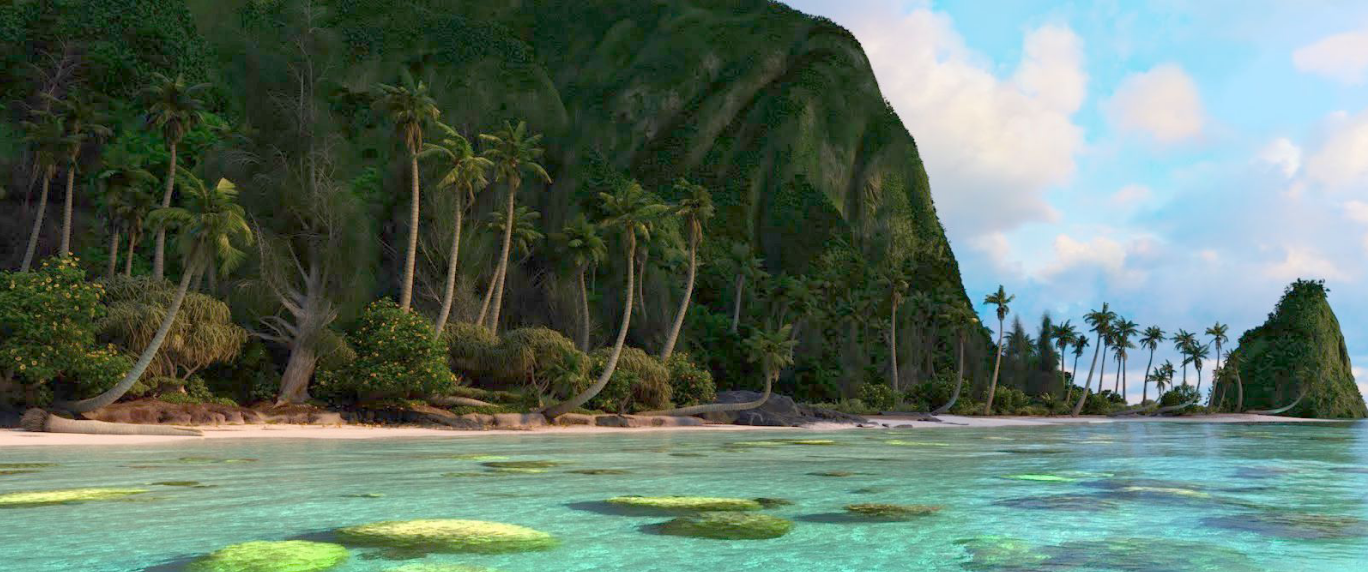
\includegraphics[width=1\linewidth]{img/concl/moana.png}
	\caption{The Moana Island Scene provided by Walt Disney Animation Studios \cite{moana2021}.}
	\label{fig:moana}
\end{figure}

\section{Future work}

\todo{traingle meshes csg'd with bvh}

\begin{figure}[!tbp]
	\centering
	\subfloat{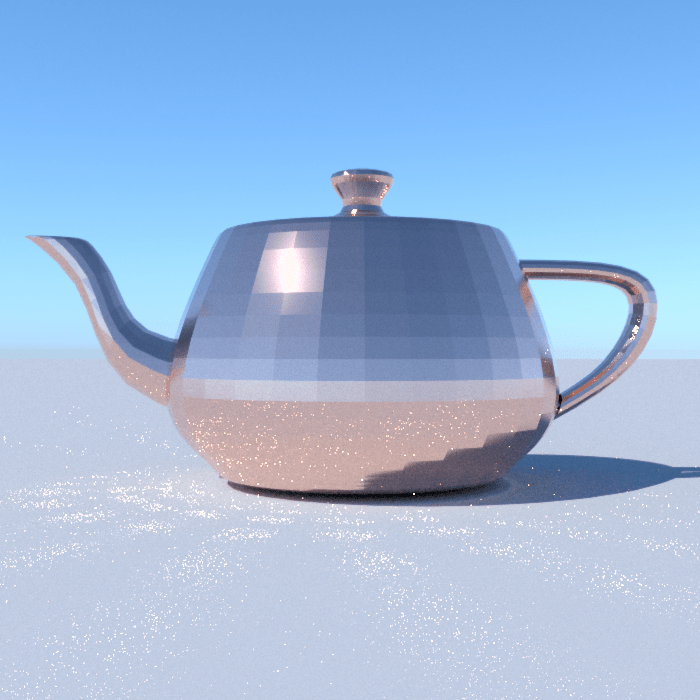
\includegraphics[width=.4\textwidth]{img/concl/teapotEmbree.png}}
	\hfill
	\subfloat{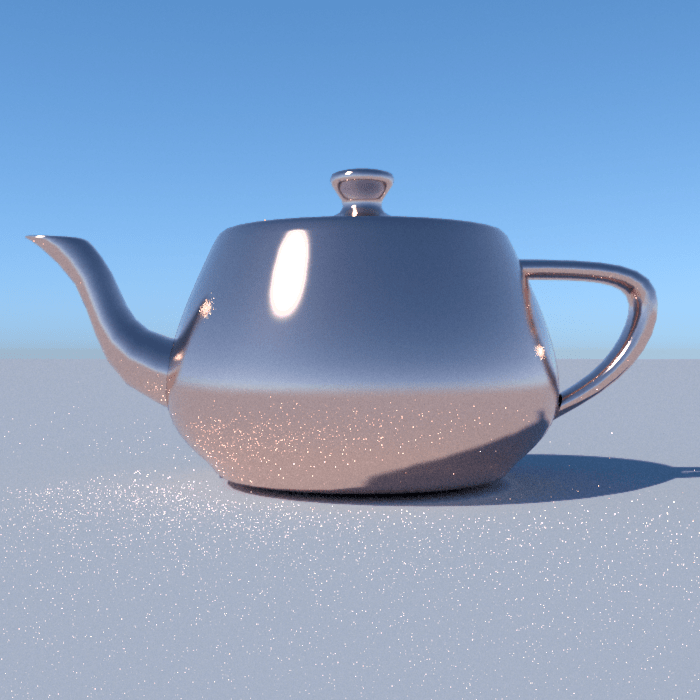
\includegraphics[width=.4\textwidth]{img/concl/teapotNormal.png}}
	\caption{Comparison between the resulting image of a scene containing the Utah teapot by ray tracing with and without Embree support.}
	\label{fig:teapot}
\end{figure}

\section{Personal note to the potential user from the author}

The main purpose of the work described in this thesis (besides the graduation of the author) is our desire to provide functionality that is of actual use for both computer graphics researchers and computer graphics enthusiasts using ART. In Chapter \ref{chap:results}, we have shown that our approach on the integration of Embree into ART accelerates the rendering process of most of the scenes on which it was tested.

We do not claim that our approach is the only way to integrate Embree into ART, nor do we claim that our implementation is the best, with regard to e.g. performance and building times of interior data structures. And although our implementation was tested on a variety of scenes, we cannot completely rule out that bugs will arise during the rendering of different scenes. Therefore we ask you to, if you encounter any issues, to report them via an email to the ART development team (the email address can be found on their website, which is \href{https://cgg.mff.cuni.cz/ART/about/}{https://cgg.mff.cuni.cz/ART/about/}). Any feedback and critique is welcomed as well. Thank you very much in advance!

We sincerely hope that our work will be useful to you!